\chapter{Configura\c c\~oes do Safari}

Este cap\'itulo traz recomenda\c c\~oes de seguran\c ca que dizem respeito ao Safari, que \'e o navegador web padr\~ao do sistema iOS. 

Analogamente \`as recomenda\c c\~oes do cap\'itulo anterior, elas impactam significamente a usabilidade do Safari. Por isso \'e recomendado consider\'a-las como medidas de defesa em profundidade e destin\'a-las apenas a dispositivos iOS nos quais a seguran\c ca \'e primordial.

\begin{figure}[h]
  \centering
  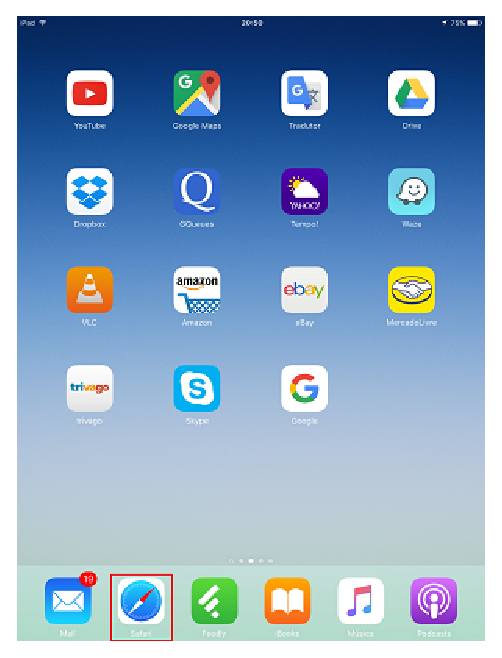
\includegraphics{imagem3.eps}
  \caption{A localiza\c c\~ao padr\~ao do \'icone do navegador Safari, destacada em vermelho}
\end{figure}

\section{Desabilitar a execu\c c\~ao de c\'odigo Javascript}

Javascript tecnologia permite que desenvolvedores de websites controlem certos elementos de p\'aginas web, como exibir a data e hora corrente, ou exibir janelas pop-up. 

Neste item, \'e recomendado que a linguagem Javascript n\~ao tenha permiss\~oes de execu\c c\~ao no navegador web padr\~ao do dispositivo, pois a mesma pode vir a ser utilizada como meio para diversos tipos de ataques aos usu\'arios. Tais ataques v\~ao desde a manipula\c c\~ao de credenciais de login at\'e a exibi\c c\~ao de p\'aginas web maliciosas, atrav\'es de janelas pop-up.

\begin{enumerate}
\item Pressionar Ajustes
\item Pressionar Safari
\item Pressionar Avan\c cado
\item Desativar Javascript, deslizando  controle para a esquerda
\end{enumerate}

\section{Habilitar o aviso de websites fraudulentos}

Este controle habilita o navegador Safari a exibir avisos e impedir o carregamento da p\'aginas de websites potencialmente fraudulentos.

Os avisos podem ajudar a evitar a visita\c c\~ao acidental a algum site de phishing, bem como outros sites desenvolvidos com inten\c c\~oes maliciosas.

\begin{enumerate}
\item Pressionar Ajustes
\item Pressionar Safari
\item Na se\c c\~ao PRIVACIDADE E SEGURAN\c CA, ativar Aviso de Site Fraudulento, deslizando o controle para a direita
\end{enumerate}

\section{Desabilitar o preenchimento autom\'atico de informa\c c\~oes de contato}

O preenchimento autom\'atico configura o navegador Safari a se lembrar de informa\c c\~oes comumente digitadas pelo usu\'ario em formul\'arios na internet, para automatizar o preenchimento de formul\'arios subsequentes.

Desabilitar o preenchimento autom\'atico ajuda a evitar o armazenamento de informa\c c\~oes sens\'iveis ou confidenciais localmente no dispositivo iOS. Tamb\'em reduz as chances de estas informa\c c\~oes serem usadas de maneira n\~ao autorizada caso alguma pessoa mal intencionada obtenha acesso ao dispositivo, seja ele um iPhone ou iPad. 

\begin{enumerate}
\item Pressionar Ajustes
\item Pressionar Safari
\item Pressionar Preenchimento Autom\'atico
\item Desativar o preenchimento autom\'atico para Dados de Contato, deslizando o controle para a esquerda
\end{enumerate}

\section{Desabilitar preenchimento autom\'atico de nomes e senhas}

O preenchimento autom\'atico configura o navegador Safari a se lembrar de credenciais, que geralmente s\~ao confidenciais, para automatizar o preenchimento de formul\'arios subsequentes.

Desabilitar o preenchimento autom\'atico ajuda a evitar o armazenamento de informa\c c\~oes sens\'iveis ou confidenciais localmente no dispositivo iOS. Tamb\'em reduz as chances de estas informa\c c\~oes serem usadas de maneira n\~ao autorizada caso alguma pessoa mal intencionada obtenha acesso ao dispositivo, seja ele um iPhone ou iPad. 

\begin{enumerate}
\item Pressionar Ajustes
\item Pressionar Safari
\item Pressionar Preenchimento Autom\'atico
\item Desativar o preenchimento autom\'atico para Nomes e Senhas, deslizando o controle para a esquerda
\end{enumerate}

\section{Desabilitar o preenchimento autom\'atico de cart\~oes de cr\'edito}

O preenchimento autom\'atico configura o navegador Safari a se lembrar de n\'umeros de cart\~oes de cr\'edito, para automatizar o preenchimento de formul\'arios subsequentes.

Desabilitar o preenchimento autom\'atico ajuda a evitar o armazenamento de n\'umeros de cart\~oes de cr\'edito localmente no dispositivo iOS. Tamb\'em reduz as chances de estas informa\c c\~oes serem usadas de maneira n\~ao autorizada caso alguma pessoa mal intencionada obtenha acesso ao dispositivo, seja ele um iPhone ou iPad. 

\begin{enumerate}
\item Pressionar Ajustes
\item Pressionar Safari
\item Pressionar Preenchimento Autom\'atico
\item Desativar o preenchimento autom\'atico para Cart\~oes de Cr\'edito, deslizando o controle para a esquerda
\end{enumerate}

\section{Apagar informa\c c\~oes sobre senhas armazenadas}

O navegador Safari fornece um reposit\'orio para armazenar informa\c c\~oes, incluindo logins e senhas, que por sua vez d\~ao suporte ao recurso de  preenchimento autom\'atico de formul\'arios. Senhas salvas s\~ao armazenadas no ``chaveiro'' do iCloud ou do dispositivo iOS, seja ele um iPhone ou iPad. 

Excluir informa\c c\~oes a respeito de credenciais salvas ajuda a impedir o uso delas, em caso de acessos n\~ao autorizados ao dispositivo.

\begin{enumerate}
\item Pressionar Ajustes
\item Pressionar Safari
\item Pressionar Senhas
\item Digitar a senha de desbloqueio do dispositivo, caso seja necess\'ario
\item Na tela seguinte, pressionar Editar
\item Pressionar cada credencial exibida, de modo a selecion\'a-las para remo\c c\~ao
\item Pressionar Apagar
\item Confirmar a remo\c c\~ao das senhas 
\end{enumerate}

\section{Remover informa\c c\~oes armazenadas sobre cart\~oes de cr\'edito}

O navegador Safari fornece um reposit\'orio para armazenar informa\c c\~oes, incluindo cart\~oes de cr\'edito, que por sua vez d\~ao suporte ao recurso de  preenchimento autom\'atico de formul\'arios. N\'umeros de cart\~oes de cr\'edito s\~ao armazenados no ``chaveiro'' do iCloud ou do dispositivo iOS, seja ele um iPhone ou iPad. 

Excluir informa\c c\~oes a respeito de cart\~oes de cr\'edito ajuda a impedir o uso deles, em caso de acessos n\~ao autorizados ao dispositivo.

\begin{enumerate}
\item Pressionar Ajustes
\item Pressionar Safari
\item Pressionar Preenchimento Autom\'atico
\item Pressionar Cart\~oes de Cr\'edito Salvos
\item Digitar a senha de desbloqueio do dispositivo, caso seja necess\'ario
\item Na tela seguinte, pressionar Editar
\item Pressionar cada cart\~ao de cr\'edito exibido, de modo a selecion\'a-los para remo\c c\~ao
\item Pressionar Apagar
\item Confirmar a remo\c c\~ao dos cart\~oes de cr\'edito 
\end{enumerate}	

\section{Habilitar a navega\c c\~ao privada}

Habilitar a navega\c c\~ao privada previne o rastreamento do hist\'orico de páginas web visitadas, pesquisas realizadas, e algumas informa\c c\~oes utilizadas pelo preenchimento autom\'atico de formul\'arios.

Habilit\'a-la pode proteger determinadas informa\c c\~oes privadas contra uso indevido e impedir alguns sites de rastrear atividades do usu\'ario atrav\'es navegador Safari.

\begin{enumerate}
\item Executar o Safari
\item Pressionar o bot\~ao de abas do Safari. No iPhone ele encontra-se no canto inferior direito do Safari. No iPad ele encontra-se no canto superior direito. 
\item Pressionar Privado
\end{enumerate}

\section{Impedir o rastreamento durante a navega\c c\~ao}

Essa configura\c c\~ao instrui o navegador Safari a comunicar, para os sites aos quais ele se conecta, que n\~ao quer ser rastreado.

Tecnicamente, quando este recurso encontra-se habilitado, o navegador Safari \'e instru\'ido a enviar um cabe\c calho opcional em requisi\c c\~oes HTTP realizadas a partir do navegador. Tal cabe\c calho indica uma prefer\^encia de n\~ao ser rastreado por sites web; por\'em, ele possui natureza volunt\'aria, ou seja, n\~ao h\'a m\'etodo ou t\'ecnica dispon\'ivel para garantir que os sites web sejam aderentes ao mesmo. Assim, ele n\~ao fornece nenhuma garantia de que sites honrar\~ao tal prefer\^encia pela privacidade. 

No entanto, um grande n\'umero de sites web s\~ao aderentes a esta configura\c c\~ao, h\'a certamente um benef\'icio em habilitar tal recurso.

\begin{enumerate}
\item Pressionar Ajustes
\item Pressionar Safari
\item Na se\c c\~ao PRIVACIDADE E SEGURAN\c CA, ativar o recurso N\~ao Rastrear, deslizando o controle para a direita
\end{enumerate}
